\documentclass[a4paper,14pt]{extreport}

% =====Задание кодировки=====
\usepackage[utf8]{inputenc}
\usepackage[english,russian]{babel}
% ===========================



% =====Размеры полей=====
\usepackage[left=3cm, right=1.5cm, vmargin=2cm]{geometry}
% =======================



% =====Полуторный интервал=====
\linespread{1.25}
% =============================



% =====Красная строка=====
\usepackage{indentfirst}
\setlength\parindent{1.25cm}
% ========================



% =====Формат заголовков=====
\usepackage{titlesec}

\titleformat
	{\chapter}
	[block]
	{\filcenter\bfseries}
	{\thechapter}
	{1ex}{}
\titlespacing{\chapter}{0pt}{*1}{*1}

\titleformat
	{\section}
	[block]
	{\hspace{\parindent}\bfseries}
	{\thesection}
	{1ex}{}
\titlespacing{\section}{0pt}{*1}{*1}

\titleformat
	{\subsection}
	[block]
	{\hspace{\parindent}\bfseries}
	{\thesubsection}
	{1ex}{}
\titlespacing{\subsection}{0pt}{*1}{*1}

\titleformat
	{\subsubsection}
	[runin]
	{\bfseries}
	{\thesubsubsection}
	{1ex}{}[. ]
\titlespacing{\subsubsection}{1.25cm}{*1}{*1}

\titleformat
	{\paragraph}
	[runin]
	{\bfseries}
	{\theparagraph}
	{1ex}{}[. ]
\titlespacing{\paragraph}{1.25cm}{*1}{*1}

\setcounter{secnumdepth}{3}
% ===========================



% =====Содержание=====
\addto{\captionsrussian}{\renewcommand*{\contentsname}{СОДЕРЖАНИЕ}}
\usepackage{titletoc}
\dottedcontents{chapter}[0em]{\bfseries}{1em}{1ex}
\dottedcontents{section}[2em]{}{2em}{1ex}
\dottedcontents{subsection}[5em]{}{3em}{1ex}
\usepackage[hidelinks]{hyperref}
% ====================



% =====Поиск по тексту=====
\usepackage{cmap}
% =========================



% =====Выравнивание текста=====
\usepackage{ragged2e}
\usepackage{microtype}
\justifying
\sloppy
\tolerance=500
\hyphenpenalty=10000
\emergencystretch=3em
% =============================



% =====Списки====
\renewcommand{\labelitemi}{--}
\renewcommand{\labelitemii}{--}

\renewcommand{\labelenumi}{\asbuk{enumi})}
\renewcommand{\labelenumii}{\arabic{enumii})}

\usepackage{enumitem}
\makeatletter
\AddEnumerateCounter{\asbuk}{\@asbuk}{ю)}
\makeatother
\setlist{nosep,wide}
\setlist[2]{labelindent=2\parindent}
% ===============



% =====Поддержка изображений и таблиц=====
\usepackage[tableposition=top,singlelinecheck=false]{caption}
\usepackage{subcaption}
\usepackage{multirow}
\usepackage{graphicx}
\usepackage{float}
\usepackage{tabularx,ragged2e,booktabs}

\DeclareCaptionLabelFormat{gostfigure}{Рисунок #2}
\DeclareCaptionLabelFormat{gosttable}{Таблица #2}
\DeclareCaptionLabelSeparator{gost}{~---~}
\captionsetup{labelsep=gost}
\captionsetup*[figure]{labelformat=gostfigure,justification=centering}
\captionsetup*[table]{labelformat=gosttable}
\renewcommand{\thesubfigure}{\asbuk{subfigure}}
% ===============================



% Запускать pdflatex с --shell-escape
% =====Листинги=====
\usepackage{minted}
% ==================



\begin{document}
	
\thispagestyle{empty}
\begin{center}

МИНИСТЕРСТВО ВЫСШЕГО ОБРАЗОВАНИЯ И НАУКИ РОССИЙСКОЙ ФЕДЕРАЦИИ
ФЕДЕРАЛЬНОЕ ГОСУДАРСТВЕННОЕ БЮДЖЕТНОЕ
ОБРАЗОВАТЕЛЬНОЕ УЧРЕЖДЕНИЕ
ВЫСШЕГО ОБРАЗОВАНИЯ

«НОВОСИБИРСКИЙ ГОСУДАРСТВЕННЫЙ ТЕХНИЧЕСКИЙ УНИВЕРСИТЕТ»

\noindent\rule{\textwidth}{0.4pt}

Кафедра вычислительной техники

\begin{figure}[H]
	\centering
	
\includegraphics{title/logo.jpeg}
\end{figure}

Лабораторная работа №3

По дисциплине: «Программное обеспечение информационных систем»

По теме: «Приложение ASP.NET Core для работы с базой данных PostgreSQL»

\end{center}

\noindent\begin{tabular}{p{0.5\textwidth}p{0.5\textwidth}}
	Выполнили: & Проверил: \\
	Студенты гр. <<АВТ-818>>, <<АВТФ>> & << должность >>\\
	<<Жигулин И. О.>> & <<Бычков М. И.>> \\
	<<Сороковикова Е. В.>> & \\
	<<\rule{1.5em}{0.4pt}>> \rule{5em}{0.4pt} 20\rule{1.5em}{0.4pt}г. & <<\rule{1.5em}{0.4pt}>> \rule{5em}{0.4pt} 20\rule{1.5em}{0.4pt}г.\\
	\rule{7.5em}{0.4pt} & \rule{7.5em}{0.4pt} \\
	\hspace{1.5em}(подпись) & \hspace{1.5em}(подпись)
\end{tabular}


\begin{center}

\vspace{2.3cm}

Новосибирск

2021
\end{center}


\tableofcontents

\chapter{Введение}

\section{Цель работы}

\begin{itemize}
	\item получить базовые навыки работы в среде R;
	\item изучить средства R для проведения первичного разведочного анализа данных (методы визуализации, описательной статистики, корреляционного анализа данных) на примере решения конкретной задачи ИАД (интеллектуального анализа данных).
\end{itemize}


\section{Задание для варианта №5}
Изучаются показатели работы программистов крупной организации. Рассматриваются следующие показатели (признаки) для каждого программиста:

\begin{itemize}
	\item пол (1-м, 2-ж);
	\item возраст;
	\item стаж работы;
	\item процент разработок, выполненных в срок в рамках бюджета с требуемым функционалом (за год);
	\item количество ошибок, выявленных пользователем (за год);
	\item стаж работы по специальности в данной организации;
	\item степень удовлетворенности заказчика;
	\item качество документирования (1 – низкое, 2 – среднее, 3 – выше среднего, 4- высокое).
\end{itemize}

Необходимо провести предварительный разведочный анализ данных с целью описания характера распределения данных, выявления структуры взаимосвязей между показателями.

Программисты разбиты на две группы в зависимости от стажа работы:

\begin{itemize}
	\item 1 группа - стаж менее 4
	\item 2 группа - стаж более 4
\end{itemize}

\chapter{Анализ исходных данных}

\section{Загрузка файла с данными}

Загрузку файла с данными можно выполнить разными способами, но мы воспользуемся тем, который не требует установки дополнительных пакетов:

\begin{minted}[fontsize=\small]{r}
data <- read.table(file      = "data.csv",
                   header    = TRUE,
                   sep       = ";",
                   row.names = 1)
\end{minted}

У загруженных данных есть один недостаток -- неудобные длинные имена для столбцов. Однако, это можно исправить с помощью следующей команды:

\begin{minted}[fontsize=\small]{r}
names(data) <- c("Группа",
                 "Пол",
                 "Возраст",
                 "Стаж",
                 "Процент успеха",
                 "Количество ошибок",
                 "Оценка заказчика",
                 "Удовлетворенность заказчика",
                 "Качество документации")
\end{minted}

Также, согласно варианту, есть две подгруппы программистов: со стажем больше 4 лет и меньше 4 лет. Назовем первую подгруппу <<juniors>>, а вторую <<seniors>>. Проведем выборку программистов для каждой подгруппы и занесем их в соответствующие переменные:

\begin{minted}[fontsize=\small]{r}
juniors <- subset(data, data$Группа == 1)
seniors <- subset(data, data$Группа == 2)
\end{minted}

Эти группы выделены для удобства использования в дальнейшем. Вместо того, чтобы каждый раз задавать подмножество всей выборки, будем обращаться к созданным переменным.


\section{Расчет основных статистических характеристик}

К основным можно отнести такие статистические характеристики как:
\begin{itemize}
	\item среднее арифметическое;
	\item медиана;
	\item стандартное отклонение;
	\item дисперсия;
	\item абсолютное отклонение медианы;
	\item сумма;
	\item минимальное значение;
	\item максимальное значение;
	\item мода;
	\item первая квартиль;
	\item третья квартиль.
\end{itemize}

Расчет этих параметров по столбцам может сообщить важную и интересную информацию, но это не всегда так. Например, найдя сумму по столбцу <<Группа>> сложно будет получить из нее сколько-нибудь значимую информацию.

Вообще, выборка содержит следующие поля, которые стоит подвергнуть статистическому анализу:

\begin{itemize}
	\item пол (количественная);
	\item возраст (количественная);
	\item стаж (количественная);
	\item процент успеха (количественная);
	\item количество ошибок (количественная);
	\item оценка заказчика (количественная);
	\item удовлетворенность заказчика (качественная);
	\item качество документации (количественная).
\end{itemize}

Для простоты вычисления основных статистических показателей напишем функцию, которая принимает параметр из выборки и считает показатели для него, а затем возвращает вектор значений, где каждый столбец подписан нужным критерием.

\begin{minted}[fontsize=\small]{r}
get_stat <- function(x) {
	x_mean   <- mean(x)
	x_median <- median(x)
	x_sd     <- sd(x)
	x_var    <- var(x)
	x_mad    <- mad(x)
	x_sum    <- sum(x)
	x_diff   <- diff(x)
	x_min    <- min(x)
	x_max    <- max(x)
	x_q1     <- quantile(x, c(0.25, 0.75))
	x_uniq   <- unique(x)
	x_mode   <- x_uniq[which.max(tabulate(match(x, x_uniq)))]
	return(c("Среднее"                       = x_mean,
	         "Медиана"                       = x_median,
	         "Стандартное отклонение"        = x_sd,
	         "Дисперсия"                     = x_var,
	         "Абсолютное отклонение медианы" = x_mad,
	         "Сумма"                         = x_sum,
	         "Минимальное значение"          = x_min,
	         "Максимальное значение"         = x_max,
	         "Квартили"                      = x_q1,
	         "Мода"                          = x_mode))
}
\end{minted}

\newpage

\subsection{Характеристики первой группы}
К первой группе программистов (juniors) относятся те, чей стаж в компании меньше четырех лет. Размер выборки --- 100 человек.

\begin{table}[H]
	\centering
	\caption{Характеристики пола первой группы}
	\begin{tabular}{|l|c|}
		\hline
		\multicolumn{1}{|c|}{\textbf{Показатель}} & \textbf{Значение}\\ \hline
		Среднее арифметическое        & 1.4       \\ \hline
		Медиана                       & 1         \\ \hline
		Стандартное отклонение        & 0.492366  \\ \hline
		Дисперсия                      & 0.2424242 \\ \hline
		Абсолютное отклонение медианы & 0         \\ \hline
		Сумма                         & 140       \\ \hline
		Минимальное значение          & 1         \\ \hline
		Максимальное значение         & 2         \\ \hline
		Мода & 1 \\ \hline
		Первая квартиль & 1 \\ \hline
		Третья квартиль & 2 \\ \hline
	\end{tabular}
\end{table}


\begin{table}[H]
	\centering
	\caption{Характеристики возраста первой группы}
	\begin{tabular}{|l|c|}
		\hline
		\multicolumn{1}{|c|}{\textbf{Показатель}} & \textbf{Значение}\\ \hline
		Среднее арифметическое        & 28.7     \\ \hline
		Медиана                       & 29       \\ \hline
		Стандартное отклонение        & 1.666667 \\ \hline
		Дисперсия                      & 2.777778 \\ \hline
		Абсолютное отклонение медианы & 1.4826   \\ \hline
		Сумма                         & 2870     \\ \hline
		Минимальное значение          & 24       \\ \hline
		Максимальное значение         & 32       \\ \hline
		Мода & 29 \\  \hline
		Первая квартиль & 28 \\ \hline
		Третья квартиль & 30 \\ \hline
	\end{tabular}
\end{table}


\begin{table}[H]
	\centering
	\caption{Характеристики стажа первой группы}
	\begin{tabular}{|l|c|}
		\hline
		\multicolumn{1}{|c|}{\textbf{Показатель}} & \textbf{Значение}\\ \hline
		Среднее арифметическое        & 2.531     \\ \hline
		Медиана                       & 2.5       \\ \hline
		Стандартное отклонение        & 0.4970001 \\ \hline
		Дисперсия                      & 0.2470091 \\ \hline
		Абсолютное отклонение медианы & 0.59304   \\ \hline
		Сумма                         & 253.1     \\ \hline
		Минимальное значение          & 1.5       \\ \hline
		Максимальное значение         & 3.7       \\ \hline
		Мода & 2.1 \\ \hline
		Первая квартиль & 2.1 \\ \hline
		Третья квартиль & 2.9 \\ \hline
	\end{tabular}
\end{table}


\begin{table}[H]
	\centering
	\caption{Характеристики процента успеха первой группы}
	\begin{tabular}{|l|c|}
		\hline
		\multicolumn{1}{|c|}{\textbf{Показатель}} & \textbf{Значение}\\ \hline
		Среднее арифметическое        & 88.22    \\ \hline
		Медиана                       & 83       \\ \hline
		Стандартное отклонение        & 5.748219 \\ \hline
		Дисперсия                      & 33.04202 \\ \hline
		Абсолютное отклонение медианы & 5.9304   \\ \hline
		Сумма                         & 8222     \\ \hline
		Минимальное значение          & 68       \\ \hline
		Максимальное значение         & 99       \\ \hline
		Мода & 83 \\ \hline
		Первая квартиль & 78 \\ \hline
		Третья квартиль & 83 \\ \hline
	\end{tabular}
\end{table}


\begin{table}[H]
	\centering
	\caption{Характеристики количества ошибок первой группы}
	\begin{tabular}{|l|c|}
		\hline
		\multicolumn{1}{|c|}{\textbf{Показатель}} & \textbf{Значение}\\ \hline
		Среднее арифметическое        & 16.86    \\ \hline
		Медиана                       & 16       \\ \hline
		Стандартное отклонение        & 4.355468 \\ \hline
		Дисперсия                      & 18.9701  \\ \hline
		Абсолютное отклонение медианы & 4.4478   \\ \hline
		Сумма                         & 1686     \\ \hline
		Минимальное значение          & 7        \\ \hline
		Максимальное значение         & 27       \\ \hline
		Мода & 15 \\ \hline
		Первая квартиль & 14 \\ \hline
		Третья квартиль & 20 \\ \hline
	\end{tabular}
\end{table}


\begin{table}[H]
	\centering
	\caption{Характеристики оценки заказчика первой группы}
	\begin{tabular}{|l|c|}
		\hline
		\multicolumn{1}{|c|}{\textbf{Показатель}} & \textbf{Значение}\\ \hline
		Среднее арифметическое        & 70.47    \\ \hline
		Медиана                       & 71       \\ \hline
		Стандартное отклонение        & 8.586406 \\ \hline
		Дисперсия                      & 73.72636 \\ \hline
		Абсолютное отклонение медианы & 10.3782  \\ \hline
		Сумма                         & 7047     \\ \hline
		Минимальное значение          & 53       \\ \hline
		Максимальное значение         & 95       \\ \hline
		Мода & 71 \\ \hline
		Первая квартиль & 64 \\ \hline
		Третья квартиль & 77 \\ \hline
	\end{tabular}
\end{table}


\begin{table}[H]
	\centering
	\caption{Характеристики качества документации первой группы}
	\begin{tabular}{|l|c|}
		\hline
		\multicolumn{1}{|c|}{\textbf{Показатель}} & \textbf{Значение}\\ \hline
		Среднее арифметическое        & 2.47      \\ \hline
		Медиана                       & 2         \\ \hline
		Стандартное отклонение        & 0.9369519 \\ \hline
		Дисперсия                      & 0.8778788 \\ \hline
		Абсолютное отклонение медианы & 1.4826    \\ \hline
		Сумма                         & 247       \\ \hline
		Минимальное значение          & 1         \\ \hline
		Максимальное значение         & 4         \\ \hline
		Мода & 2 \\ \hline
		Первая квартиль & 2 \\ \hline
		Третья квартиль & 3 \\ \hline
	\end{tabular}
\end{table}






\subsection{Характеристики второй группы}
Ко второй группе программистов (seniors) относятся те, чей стаж в компании больше четырех лет. Размер выборки --- 100 человек.

\begin{table}[H]
	\centering
	\caption{Характеристики пола второй группы}
	\begin{tabular}{|l|c|}
		\hline
		\multicolumn{1}{|c|}{\textbf{Показатель}} & \textbf{Значение}\\ \hline
		Среднее арифметическое        & 1.45 \\ \hline
		Медиана                       & 1    \\ \hline
		Стандартное отклонение        & 0.5  \\ \hline
		Дисперсия                      & 0.25 \\ \hline
		Абсолютное отклонение медианы & 0    \\ \hline
		Сумма                         & 145  \\ \hline
		Минимальное значение          & 1    \\ \hline
		Максимальное значение         & 2    \\ \hline
		Мода & 1 \\ \hline
		Первая квартиль & 1 \\ \hline
		Третья квартиль & 2 \\ \hline
	\end{tabular}
\end{table}


\begin{table}[H]
	\centering
	\caption{Характеристики возраста второй группы}
	\begin{tabular}{|l|c|}
		\hline
		\multicolumn{1}{|c|}{\textbf{Показатель}} & \textbf{Значение}\\ \hline
		Среднее арифметическое        & 32.46    \\ \hline
		Медиана                       & 32       \\ \hline
		Стандартное отклонение        & 2.19006  \\ \hline
		Дисперсия                      & 4.796364 \\ \hline
		Абсолютное отклонение медианы & 1.4826   \\ \hline
		Сумма                         & 3246     \\ \hline
		Минимальное значение          & 26       \\ \hline
		Максимальное значение         & 37       \\ \hline
		Мода & 32 \\ \hline
		Первая квартиль & 31 \\ \hline
		Третья квартиль & 34 \\ \hline
	\end{tabular}
\end{table}


\begin{table}[H]
	\centering
	\caption{Характеристики стажа второй группы}
	\begin{tabular}{|l|c|}
		\hline
		\multicolumn{1}{|c|}{\textbf{Показатель}} & \textbf{Значение}\\ \hline
		Среднее арифметическое        & 6.377     \\ \hline
		Медиана                       & 6.35      \\ \hline
		Стандартное отклонение        & 0.7226292 \\ \hline
		Дисперсия                      & 0.5221929 \\ \hline
		Абсолютное отклонение медианы & 0.66717   \\ \hline
		Сумма                         & 637.7     \\ \hline
		Минимальное значение          & 4.9       \\ \hline
		Максимальное значение         & 8.5       \\ \hline
		Мода & 6.6 \\ \hline
		Первая квартиль & 5.8 \\ \hline
		Третья квартиль & 6.8 \\ \hline
	\end{tabular}
\end{table}


\begin{table}[H]
	\centering
	\caption{Характеристики процента успеха второй группы}
	\begin{tabular}{|l|c|}
		\hline
		\multicolumn{1}{|c|}{\textbf{Показатель}} & \textbf{Значение}\\ \hline
		Среднее арифметическое        & 88.66    \\ \hline
		Медиана                       & 82       \\ \hline
		Стандартное отклонение        & 4.31867  \\ \hline
		Дисперсия                      & 18.65091 \\ \hline
		Абсолютное отклонение медианы & 4.4478   \\ \hline
		Сумма                         & 8266     \\ \hline
		Минимальное значение          & 72       \\ \hline
		Максимальное значение         & 93       \\ \hline
		Мода & 81 \\ \hline
		Первая квартиль & 80 \\ \hline
		Третья квартиль & 86 \\ \hline
	\end{tabular}
\end{table}


\begin{table}[H]
	\centering
	\caption{Характеристики количества ошибок второй группы}
	\begin{tabular}{|l|c|}
		\hline
		\multicolumn{1}{|c|}{\textbf{Показатель}} & \textbf{Значение}\\ \hline
		Среднее арифметическое        & 13.48    \\ \hline
		Медиана                       & 14       \\ \hline
		Стандартное отклонение        & 3.817768 \\ \hline
		Дисперсия                      & 14.57535 \\ \hline
		Абсолютное отклонение медианы & 2.9652   \\ \hline
		Сумма                         & 1348     \\ \hline
		Минимальное значение          & 3        \\ \hline
		Максимальное значение         & 26       \\ \hline
		Мода & 14 \\ \hline
		Первая квартиль & 11 \\ \hline
		Третья квартиль & 16 \\ \hline
	\end{tabular}
\end{table}


\begin{table}[H]
	\centering
	\caption{Характеристики оценки заказчика второй группы}
	\begin{tabular}{|l|c|}
		\hline
		\multicolumn{1}{|c|}{\textbf{Показатель}} & \textbf{Значение}\\ \hline
		Среднее арифметическое        & 74.48    \\ \hline
		Медиана                       & 75       \\ \hline
		Стандартное отклонение        & 8.372007 \\ \hline
		Дисперсия                      & 70.09051 \\ \hline
		Абсолютное отклонение медианы & 7.413    \\ \hline
		Сумма                         & 7448     \\ \hline
		Минимальное значение          & 57       \\ \hline
		Максимальное значение         & 99       \\ \hline
		Мода & 79 \\ \hline
		Первая квартиль & 69.75 \\ \hline
		Третья квартиль & 79 \\ \hline
	\end{tabular}
\end{table}


\begin{table}[H]
	\centering
	\caption{Характеристики качества документации второй группы}
	\begin{tabular}{|l|c|}
		\hline
		\multicolumn{1}{|c|}{\textbf{Показатель}} & \textbf{Значение}\\ \hline
		Среднее арифметическое        & 2.49      \\ \hline
		Медиана                       & 3         \\ \hline
		Стандартное отклонение        & 0.9480975 \\ \hline
		Дисперсия                      & 0.8988889 \\ \hline
		Абсолютное отклонение медианы & 1.4826    \\ \hline
		Сумма                         & 249       \\ \hline
		Минимальное значение          & 1         \\ \hline
		Максимальное значение         & 4         \\ \hline
		Мода & 3 \\ \hline
		Первая квартиль & 2 \\ \hline
		Третья квартиль & 3 \\ \hline
	\end{tabular}
\end{table}







\subsection{Характеристики всей выборки}
Общая группа программистов состоит из 200 человек и не разделяется по выработанному стажу.

\begin{table}[H]
	\centering
	\caption{Характеристики пола общей группы}
	\begin{tabular}{|l|c|}
		\hline
		\multicolumn{1}{|c|}{\textbf{Показатель}} & \textbf{Значение}\\ \hline
		Среднее арифметическое        & 1.425     \\ \hline
		Медиана                       & 1         \\ \hline
		Стандартное отклонение        & 0.4955835 \\ \hline
		Дисперсия                      & 0.245603  \\ \hline
		Абсолютное отклонение медианы & 0         \\ \hline
		Сумма                         & 285       \\ \hline
		Минимальное значение          & 1         \\ \hline
		Максимальное значение         & 2         \\ \hline
		Мода & 1 \\ \hline
		Первая квартиль & 1 \\ \hline
		Третья квартиль & 2 \\ \hline
	\end{tabular}
\end{table}


\begin{table}[H]
	\centering
	\caption{Характеристики возраста общей группы}
	\begin{tabular}{|l|c|}
		\hline
		\multicolumn{1}{|c|}{\textbf{Показатель}} & \textbf{Значение}\\ \hline
		Среднее арифметическое        & 30.58    \\ \hline
		Медиана                       & 30       \\ \hline
		Стандартное отклонение        & 2.705587 \\ \hline
		Дисперсия                      & 7.320201 \\ \hline
		Абсолютное отклонение медианы & 2.9652   \\ \hline
		Сумма                         & 6116     \\ \hline
		Минимальное значение          & 24       \\ \hline
		Максимальное значение         & 37       \\ \hline
		Мода & 30 \\ \hline
		Первая квартиль & 29 \\ \hline
		Третья квартиль & 32 \\ \hline
	\end{tabular}
\end{table}


\begin{table}[H]
	\centering
	\caption{Характеристики стажа общей группы}
	\begin{tabular}{|l|c|}
		\hline
		\multicolumn{1}{|c|}{\textbf{Показатель}} & \textbf{Значение}\\ \hline
		Среднее арифметическое        & 4.454    \\ \hline
		Медиана                       & 4.3      \\ \hline
		Стандартное отклонение        & 2.024643 \\ \hline
		Дисперсия                      & 4.09918  \\ \hline
		Абсолютное отклонение медианы & 2.81694  \\ \hline
		Сумма                         & 890.8    \\ \hline
		Минимальное значение          & 1.5      \\ \hline
		Максимальное значение         & 8.5      \\ \hline
		Мода & 2.1 \\ \hline
		Первая квартиль & 2.5 \\ \hline
		Третья квартиль & 6.325 \\ \hline
	\end{tabular}
\end{table}


\begin{table}[H]
	\centering
	\caption{Характеристики процента успеха общей группы}
	\begin{tabular}{|l|c|}
		\hline
		\multicolumn{1}{|c|}{\textbf{Показатель}} & \textbf{Значение}\\ \hline
		Среднее арифметическое        & 82.44    \\ \hline
		Медиана                       & 83       \\ \hline
		Стандартное отклонение        & 5.075946 \\ \hline
		Дисперсия                      & 25.76523 \\ \hline
		Абсолютное отклонение медианы & 4.4478   \\ \hline
		Сумма                         & 16488    \\ \hline
		Минимальное значение          & 68       \\ \hline
		Максимальное значение         & 99       \\ \hline
		Мода & 81 \\ \hline
		Первая квартиль & 79 \\ \hline
		Третья квартиль & 86 \\ \hline
	\end{tabular}
\end{table}


\begin{table}[H]
	\centering
	\caption{Характеристики количества ошибок общей группы}
	\begin{tabular}{|l|c|}
		\hline
		\multicolumn{1}{|c|}{\textbf{Показатель}} & \textbf{Значение}\\ \hline
		Среднее арифметическое        & 15.17    \\ \hline
		Медиана                       & 15       \\ \hline
		Стандартное отклонение        & 4.422544 \\ \hline
		Дисперсия                      & 19.55889 \\ \hline
		Абсолютное отклонение медианы & 4.4478   \\ \hline
		Сумма                         & 3034     \\ \hline
		Минимальное значение          & 3        \\ \hline
		Максимальное значение         & 27       \\ \hline
		Мода & 15 \\ \hline
		Первая квартиль & 12 \\ \hline
		Третья квартиль & 18 \\ \hline
	\end{tabular}
\end{table}


\begin{table}[H]
	\centering
	\caption{Характеристики оценки заказчика общей группы}
	\begin{tabular}{|l|c|}
		\hline
		\multicolumn{1}{|c|}{\textbf{Показатель}} & \textbf{Значение}\\ \hline
		Среднее арифметическое        & 72.475   \\ \hline
		Медиана                       & 73       \\ \hline
		Стандартное отклонение        & 8.694096 \\ \hline
		Дисперсия                      & 75.58731 \\ \hline
		Абсолютное отклонение медианы & 8.8956   \\ \hline
		Сумма                         & 14495    \\ \hline
		Минимальное значение          & 53       \\ \hline
		Максимальное значение         & 99       \\ \hline
		Мода & 79 \\ \hline
		Первая квартиль & 66 \\ \hline
		Третья квартиль & 79 \\ \hline
	\end{tabular}
\end{table}


\begin{table}[H]
	\centering
	\caption{Характеристики качества документации общей группы}
	\begin{tabular}{|l|c|}
		\hline
		\multicolumn{1}{|c|}{\textbf{Показатель}} & \textbf{Значение}\\ \hline
		Среднее арифметическое        & 2.48      \\ \hline
		Медиана                       & 3         \\ \hline
		Стандартное отклонение        & 0.9402234 \\ \hline
		Дисперсия                      & 0.8830201 \\ \hline
		Абсолютное отклонение медианы & 1.4826    \\ \hline
		Сумма                         & 496       \\ \hline
		Минимальное значение          & 1         \\ \hline
		Максимальное значение         & 4         \\ \hline
		Мода & 3 \\ \hline
		Первая квартиль & 2 \\ \hline
		Третья квартиль & 3 \\ \hline
	\end{tabular}
\end{table}


\subsection{Характеристики качественных данных}
Не все столбцы в наборе данных являются количественными. Так, например, столбец <<Удовлетворенность заказчика>> относится к качественным данным. Чтобы работать с таким типом данных, необходимо каким-либо образом трансформировать его в количественный.

В нашем случае, можно заметить, что данные в столбце <<Удовлетворенность заказчика>> принимают всего три значения:
\begin{itemize}
	\item низкая;
	\item средняя;
	\item высокая.
\end{itemize}

Трансформация таких данных не вызывает особых трудностей. Их можно отобразить на множество $\{1, 2, 3\}$ соответственно. После этого к ним можно применить точно такие же функции, что и к количественным данным.

Преобразование можно выполнить с помощью следующих команд:
\begin{minted}[fontsize=\small]{r}
index <- data$`Удовлетворенность заказчика` == "низкая"
data[index, "Удовлетворенность заказчика"] <- as.numeric(1)
index <- data$`Удовлетворенность заказчика` == "средняя"
data[index, "Удовлетворенность заказчика"] <- as.numeric(2)
index <- data$`Удовлетворенность заказчика` == "высокая"
data[index, "Удовлетворенность заказчика"] <- as.numeric(3)
data[, "Удовлетворенность заказчика"] <- 
    as.numeric(data[, "Удовлетворенность заказчика"])
\end{minted}

\begin{table}[H]
	\centering
	\caption{Характеристики удовлетворенности заказчика первой группы}
	\begin{tabular}{|l|c|}
		\hline
		\multicolumn{1}{|c|}{\textbf{Показатель}} & \textbf{Значение}\\ \hline
		Среднее арифметическое        & 2.03      \\ \hline
		Медиана                       & 2         \\ \hline
		Стандартное отклонение        & 0.797154  \\ \hline
		Дисперсия                      & 0.6354545 \\ \hline
		Абсолютное отклонение медианы & 1.4826    \\ \hline
		Сумма                         & 203       \\ \hline
		Минимальное значение          & 1         \\ \hline
		Максимальное значение         & 3         \\ \hline
		Мода & 2 \\ \hline
		Первая квартиль & 1 \\ \hline
		Третья квартиль & 3 \\ \hline
	\end{tabular}
\end{table}

\begin{table}[H]
	\centering
	\caption{Характеристики удовлетворенности заказчика второй группы}
	\begin{tabular}{|l|c|}
		\hline
		\multicolumn{1}{|c|}{\textbf{Показатель}} & \textbf{Значение}\\ \hline
		Среднее арифметическое        & 2.31      \\ \hline
		Медиана                       & 2         \\ \hline
		Стандартное отклонение        & 0.747994  \\ \hline
		Дисперсия                      & 0.5594949 \\ \hline
		Абсолютное отклонение медианы & 1.4826    \\ \hline
		Сумма                         & 231       \\ \hline
		Минимальное значение          & 1         \\ \hline
		Максимальное значение         & 3         \\ \hline
		Мода & 3 \\ \hline
		Первая квартиль & 2 \\ \hline
		Третья квартиль & 3 \\ \hline
	\end{tabular}
\end{table}

\begin{table}[H]
	\centering
	\caption{Характеристики удовлетворенности заказчика общей группы}
	\begin{tabular}{|l|c|}
		\hline
		\multicolumn{1}{|c|}{\textbf{Показатель}} & \textbf{Значение}\\ \hline
		Среднее арифметическое        & 2.17      \\ \hline
		Медиана                       & 2         \\ \hline
		Стандартное отклонение        & 0.7836905 \\ \hline
		Дисперсия                      & 0.6141709 \\ \hline
		Абсолютное отклонение медианы & 1.4826    \\ \hline
		Сумма                         & 434       \\ \hline
		Минимальное значение          & 1         \\ \hline
		Максимальное значение         & 3         \\ \hline
		Мода & 3 \\ \hline
		Первая квартиль & 2 \\ \hline
		Третья квартиль & 2 \\ \hline
	\end{tabular}
\end{table}





\subsection{Выводы}
Анализируя полученные результаты можно сделать следующие выводы:

\begin{enumerate}
	\item Во обоих группах гендерное распределение склоняется в сторону мужчин. В группе juniors 60\% мужчин и 40\% женщин, а в группе seniors 55\% мужчин и 45\% женщин. Всего среди программистов представленных в выборке 42.5\% женщин и 57.5\% мужчин.
	
	\item Средний возраст программистов в общем -- 30.58 лет. В группе juniors -- 28.7 лет, а в группе seniors -- 32.46 лет. При этом разброс возрастов для группы seniors лежит на отрезке от 26 до 37 лет. Для группы juniors -- на отрезке от 24 до 32 лет. Суммарно все программисты прожили 6116 лет.
	
	\item В среднем люди проработали в компании 4.454 года. При этом самый последний программист был нанят 1.5 года назад, а самый <<старый>> 8.5 лет назад.Суммарно все программисты посвятили компании 890.8 лет.
	
	\item Группа juniors закрывает успешно 88.22\% задач за год. Самый неэффективный работник по этой метрике закрывает 68\% задач, а самый эффективный -- 99\%. В группе seniors успешно выполняется 88.66\% задач. Диапазон эффективности от 72\% до 93\%. В общем все программисты работают с эффективностью 82.44\%. Процент закрытия задач примерно одинаков, однако важно понимать, что, скорее всего, более опытные разработчики реализуют гараздо более сложные и важные задачи. Также человек с самым низким показателем не обязательно является лентяем. Вполне вероятно, что часть задач, которые он решал потребовали от него гораздо больше времени и сил на решение из-за чего он не смог закрыть остальные.
	
	\item Количество ошибок, которые допускают программисты колеблется от 3 до 27. Всего за год обнаруживается 3034 ошибки. В среднем на каждого программиста приходится по 15.17 ошибки. В группе siniors в среднем обнаруживается 13.48 ошибки. При этом максимальное количество допущенных ошибок 1 программистом равно 26. В группе juniors в среднем допускается 16.86 ошибки в год. При этом минимальное количество ошибок равно 7 против 3 у группы seniors. Все допускают ошибки, но явно видно, что опыт сказывается, и разработчики со стажем допускают меньше ошибок.
	
	\item Заказчик оценивает работу программиста в среднем на 72.475 балла из 100. Самая низкая оценка от заказчика -- 53, а самая высокая 99. В группе juniors средняя оценка составляет 70.47 баллов, а в группе seniors -- 74.48 балла. Из чего может следовать, что группа seniors выполняет свою работу несколько лучше.
	
	\item Заказчик в общем удовлетворен чуть выше среднего.
	
	\item Качество документации в среднем составляет 2.48 балла. Максимальная оценка за документацию равна 4, а минимальная -- 1. Можно сказать, что разработчики не особо стремятся составлять документацию к производимым продуктам.
\end{enumerate}











\section{Графический анализ данных}

\subsection{Графики}

\begin{figure}[H]
	\centering
	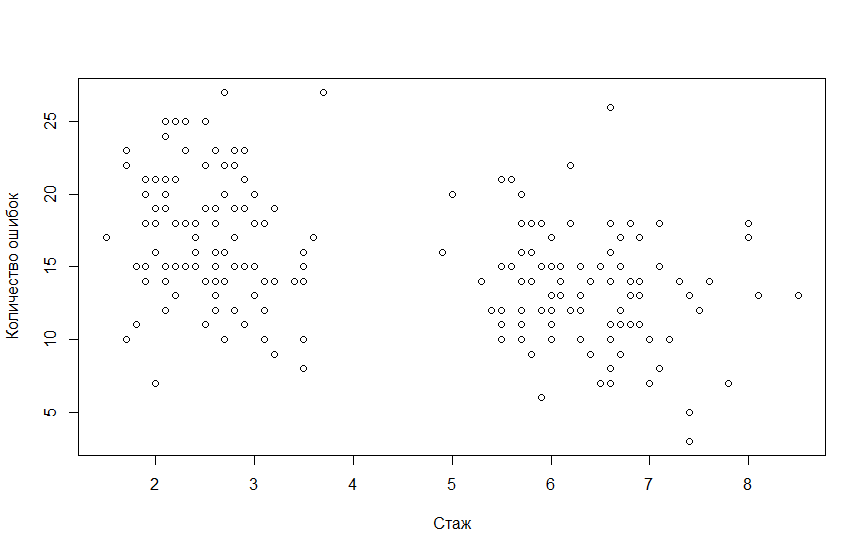
\includegraphics[width=\linewidth]{fig3}
	\caption{Диаграмма рассеяния по двум количественным признакам}
\end{figure}

\begin{figure}[H]
	\centering
	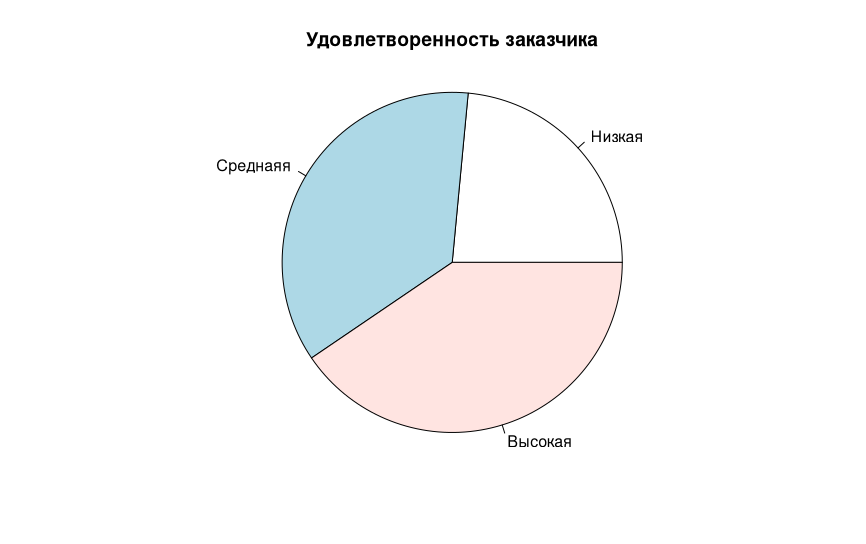
\includegraphics[width=\linewidth]{fig2}
	\caption{Радиальная диаграмма по качественному признаку}
\end{figure}




\begin{figure}[H]
	\centering
	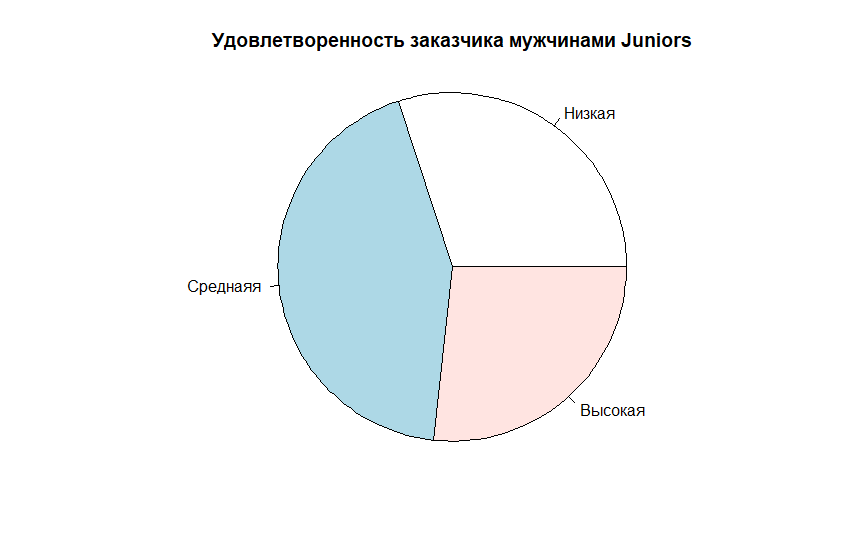
\includegraphics[width=\linewidth]{figmj}
	\caption{Удовлетворенность заказчика мужчинами <<juniors>>}
\end{figure}

\begin{figure}[H]
	\centering
	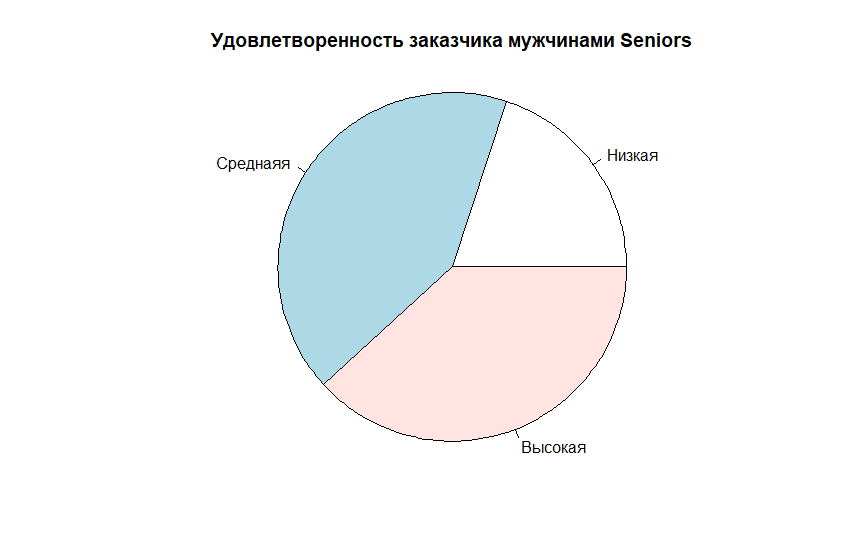
\includegraphics[width=\linewidth]{figms}
	\caption{Удовлетворенность заказчика мужчинами <<seniors>>}
\end{figure}

\begin{figure}[H]
	\centering
	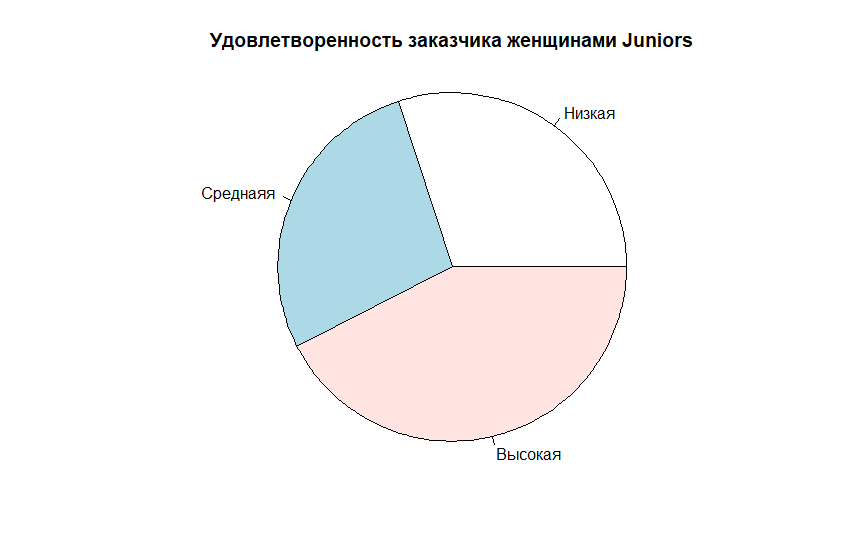
\includegraphics[width=\linewidth]{figwj}
	\caption{Удовлетворенность заказчика женщинами <<juniors>>}
\end{figure}

\begin{figure}[H]
	\centering
	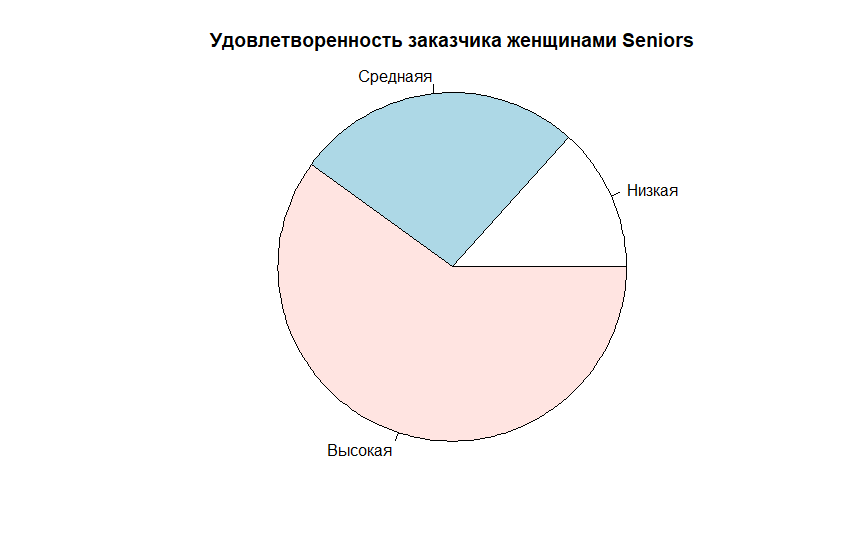
\includegraphics[width=\linewidth]{figws}
	\caption{Удовлетворенность заказчика женщинами <<seniors>>}
\end{figure}

\begin{figure}[H]
	\centering
	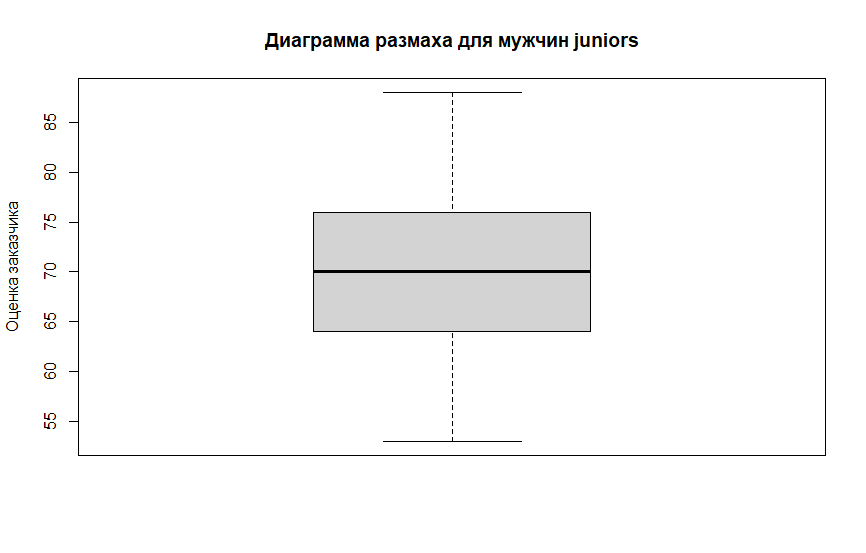
\includegraphics[width=\linewidth]{figboxmj}
	\caption{Оценка заказчика мужчин <<juniors>>}
\end{figure}

\begin{figure}[H]
	\centering
	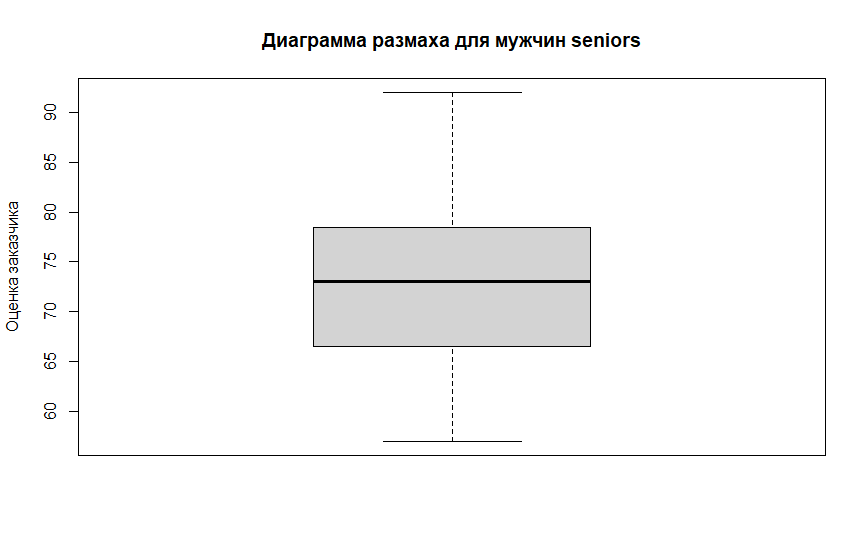
\includegraphics[width=\linewidth]{figboxms}
	\caption{Оценка заказчика мужчин <<seniors>>}
\end{figure}

\begin{figure}[H]
	\centering
	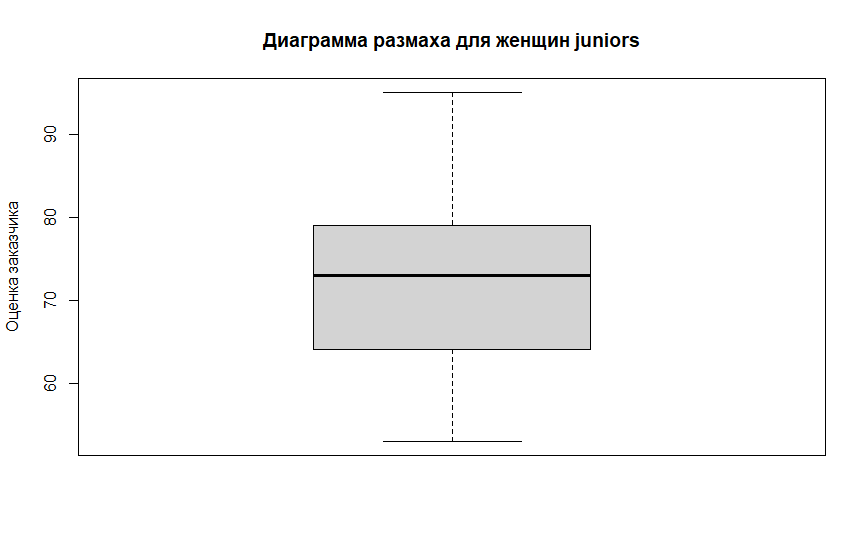
\includegraphics[width=\linewidth]{figboxwj}
	\caption{Оценка заказчика женщин <<juniors>>}
\end{figure}

\begin{figure}[H]
	\centering
	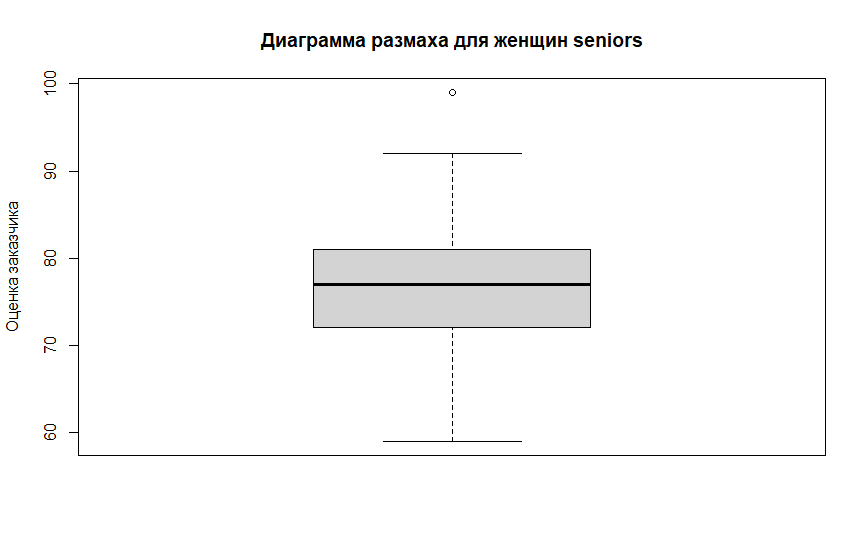
\includegraphics[width=\linewidth]{figboxws}
	\caption{Оценка заказчика женщин <<seniors>>}
\end{figure}

\begin{figure}[H]
	\centering
	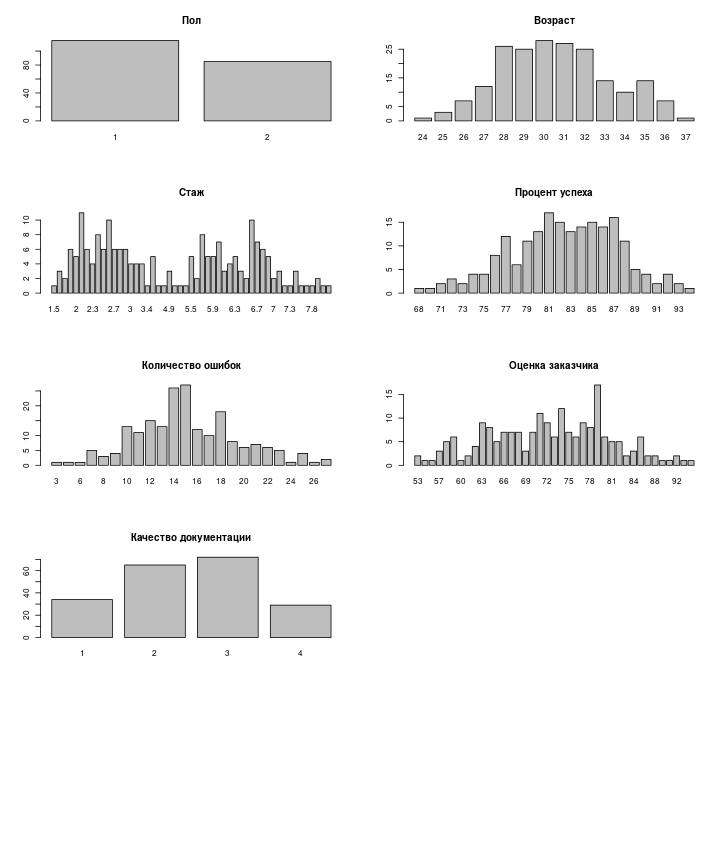
\includegraphics[width=\linewidth]{fighist}
	\caption{Гистограммы для всех количественных признаков}
\end{figure}

\begin{figure}[H]
	\centering
	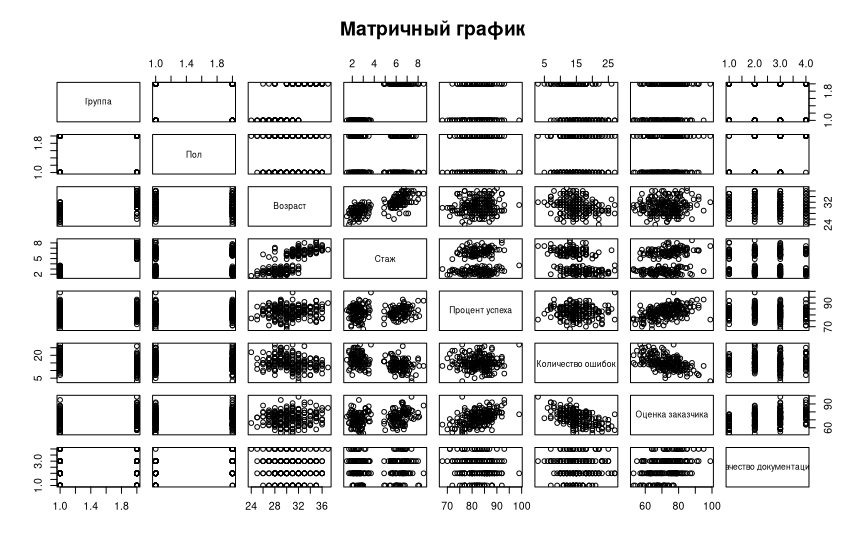
\includegraphics[width=\linewidth]{fig1}
	\caption{Матричный график по всем количественным переменным}
\end{figure}

\subsection{Выводы}

Анализируя графики, можно сделать следующие выводы:

\begin{itemize}
	\item На работе шире представлены мужчины.
	\item Больше всего программистов находятся в возрастном диапазоне от 28 до 32.
	\item Наиболее частые проценты успеха лежат на отрезке от 81 до 87.
	\item График количества ошибок схож с графиком нормального распределения.
	\item Заказчики чаще всего ставят оценку от 78 до 81.
	\item Качество документации можно оценить как <<чуть ниже среднего>>.
	\item Удовлетворенность заказчиков работой женщин значительно выше, чем удовлетворенность работой мужчин. Возможно, это можно списать на заниженные ожидания из-за стереотипного отношения к женщинам. Ведь в целом, женщины и мужчины не сильно отличаются по качеству и эффективности работы.
\end{itemize}












\section{Корреляционный анализ данных}

\subsection{Коэффициенты корреляции Пирсона, Спирмена и Кендала}

Для оценки степени взаимосвязи между количественными переменными на основе коэффициентов Пирсона, Спирмена и Кендалла напишем следующий код:

\begin{minted}[fontsize=\small]{r}
MJ <- juniors[, unlist(lapply(juniors, is.numeric))]
MS <- seniors[, unlist(lapply(seniors, is.numeric))]

JP <- cor(MJ, use = "all.obs")
JS <- cor(MJ, use = "all.obs", method = "spearman")
JK <- cor(MJ, use = "all.obs", method = "kendall")

SP <- cor(MS, use = "all.obs")
SS <- cor(MS, use = "all.obs", method = "spearman")
SK <- cor(MS, use = "all.obs", method = "kendall")
\end{minted}



\paragraph{Первая группа}
Данные для первой группы (<<juniors>>) представлены в таблицах \ref{jun/p} -- \ref{jun/k}.

\begin{table}[H]
	\centering
	\caption{Критерий Пирсона для группы <<juniors>>}
	\begin{tabular}{|l|c|c|c|c|c|c|}
		\hline
		&  
		\begin{sideways}
			Возраст
		\end{sideways}  & 
		\begin{sideways}
			Стаж
		\end{sideways} & 
		\begin{sideways}
			Процент успеха
		\end{sideways} & 
		\begin{sideways}
			Количество ошибок
		\end{sideways} &
		\begin{sideways}
			Оценка заказчика
		\end{sideways} & 
		\begin{sideways}
			Качество документации~
		\end{sideways} \\ \hline
		Пол                   & -0.21 & -0.20 & -0.01 & 0.09 & 0.10 & 0.42 \\ \hline
		Возраст               && 0.32 & 0.01 & 0.10 & -0.11 & -0.14 \\\hline
		Стаж                  &&&  0.15 & -0.13 &  0.12 & -0.12 \\ \hline
		Процент успеха        &&&& -0.04 &  0.59 & -0.11 \\ \hline
		Количество ошибок     &&&&& -0.47 &  0.14 \\ \hline
		Оценка заказчика      &&&&&&  0.26 \\ \hline
	\end{tabular}
	\label{jun/p}
\end{table}

\begin{table}[H]
	\centering
	\caption{Критерий Спирмена для группы <<juniors>>}
	\begin{tabular}{|l|c|c|c|c|c|c|}
		\hline
		& 
		\begin{sideways}
			Возраст
		\end{sideways}  & 
		\begin{sideways}
			Стаж
		\end{sideways} & 
		\begin{sideways}
			Процент успеха
		\end{sideways} & 
		\begin{sideways}
			Количество ошибок
		\end{sideways} &
		\begin{sideways}
			Оценка заказчика
		\end{sideways} & 
		\begin{sideways}
			Качество документации~
		\end{sideways} \\ \hline
		Пол                   & -0.19 & -0.20 & -0.01 & 0.08 & 0.10 & 0.40 \\ \hline
		Возраст               &&  0.29 & -0.03 &  0.12 & -0.12 & -0.09 \\ \hline	
		Стаж                  &&&  0.09 & -0.14 &  0.11 & -0.14 \\ \hline
		Процент успеха        &&&& -0.08 &  0.59 & -0.11 \\ \hline
		Количество ошибок     &&&&& -0.48 &  0.12 \\ \hline	
		Оценка заказчика      &&&&&&  0.24 \\ \hline	
	\end{tabular}
	\label{jun/s}
\end{table}

\begin{table}[H]
	\centering
	\caption{Критерий Кенделла для группы <<juniors>>}
	\begin{tabular}{|l|c|c|c|c|c|c|}
		\hline
		&  
		\begin{sideways}
			Возраст
		\end{sideways}  & 
		\begin{sideways}
			Стаж
		\end{sideways} & 
		\begin{sideways}
			Процент успеха
		\end{sideways} & 
		\begin{sideways}
			Количество ошибок
		\end{sideways} &
		\begin{sideways}
			Оценка заказчика
		\end{sideways} & 
		\begin{sideways}
			Качество документации~
		\end{sideways} \\ \hline
		Пол                   & -0.17 & -0.17 & -0.01 & 0.06 & 0.08 & 0.37 \\\hline
		Возраст               &&  0.22 & -0.02 &  0.09 & -0.09 & -0.08 \\ \hline
		Стаж                  &&&  0.06 & -0.10 &  0.07 & -0.11 \\ \hline
		Процент успеха        &&&& -0.06 &  0.43 & -0.08 \\ \hline	
		Количество ошибок     &&&&& -0.35 &  0.09 \\ \hline	
		Оценка заказчика      &&&&&&  0.18 \\ \hline	
	\end{tabular}
	\label{jun/k}
\end{table}




\paragraph{Вторая группа}
Данные для второй группы (<<seniors>>) представлены в таблицах \ref{sen/p} -- \ref{sen/k}.

\begin{table}[H]
	\centering
	\caption{Критерий Пирсона для группы <<seniors>>}
	\begin{tabular}{|l|c|c|c|c|c|c|}
		\hline
		& 
		\begin{sideways}
			Возраст
		\end{sideways}  & 
		\begin{sideways}
			Стаж
		\end{sideways} & 
		\begin{sideways}
			Процент успеха
		\end{sideways} & 
		\begin{sideways}
			Количество ошибок
		\end{sideways} &
		\begin{sideways}
			Оценка заказчика
		\end{sideways} & 
		\begin{sideways}
			Качество документации~
		\end{sideways} \\ \hline
		Пол                   & 0.03 & 0.09 & -0.02 & 0.03 & 0.21 & 0.51 \\ \hline
		Возраст               && 0.46 & 0.17 & -0.01 & -0.04 & -0.04  \\ \hline	
		Стаж                  &&& 0.29 & -0.21 & 0.34 & 0.10  \\ \hline
		Процент успеха        &&&& 0.06 & 0.37 & -0.01  \\ \hline
		Количество ошибок     &&&&& -0.53 & -0.13  \\ \hline	
		Оценка заказчика      &&&&&& 0.50  \\ \hline
	\end{tabular}
	\label{sen/p}
\end{table}

\begin{table}[H]
	\centering
	\caption{Критерий Спирмена для группы <<seniors>>}
	\begin{tabular}{|l|c|c|c|c|c|c|}
		\hline
		&
		\begin{sideways}
			Возраст
		\end{sideways}  & 
		\begin{sideways}
			Стаж
		\end{sideways} & 
		\begin{sideways}
			Процент успеха
		\end{sideways} & 
		\begin{sideways}
			Количество ошибок
		\end{sideways} &
		\begin{sideways}
			Оценка заказчика
		\end{sideways} & 
		\begin{sideways}
			Качество документации~
		\end{sideways} \\ \hline
		Пол                   & 0.01 & 0.11 & -0.02 & 0.01  & 0.22 & 0.39 \\ \hline
		Возраст               && 0.49 & 0.21 & 0.02 & -0.04 & -0.06  \\ \hline	
		Стаж                  &&& 0.25 & -0.19 & 0.34 & 0.12  \\ \hline
		Процент успеха        &&&& 0.07 & 0.41 & -0.01  \\ \hline
		Количество ошибок     &&&&& -0.46 & -0.12  \\ \hline	
		Оценка заказчика      &&&&&& 0.48  \\ \hline
	\end{tabular}
	\label{sen/s}
\end{table}

\begin{table}[H]
	\centering
	\caption{Критерий Кенделла для группы <<seniors>>}
	\begin{tabular}{|l|c|c|c|c|c|c|}
		\hline
		&
		\begin{sideways}
			Возраст
		\end{sideways}  & 
		\begin{sideways}
			Стаж
		\end{sideways} & 
		\begin{sideways}
			Процент успеха
		\end{sideways} & 
		\begin{sideways}
			Количество ошибок
		\end{sideways} &
		\begin{sideways}
			Оценка заказчика
		\end{sideways} & 
		\begin{sideways}
			Качество документации~
		\end{sideways} \\ \hline
		Пол                   & 0.01 & 0.09 & -0.02 & 0.01 & 0.18 & 0.45  \\ \hline
		Возраст               && 0.37 & 0.16  & 0.01 & -0.03 & -0.04  \\ \hline
		Стаж                  &&&  0.19 & -0.14  &0.23  &  0.10 \\ \hline
		Процент успеха        &&&& 0.05 & 0.30 &  -0.01 \\ \hline
		Количество ошибок     &&&&& -0.34 & -0.10 \\ \hline
		Оценка заказчика      &&&&&& 0.37  \\ \hline 	
	\end{tabular}
	\label{sen/k}
\end{table}


\subsection{Частный коэффициент корреляции}
Для вычисления частного коэффициента корреляции будет использоваться следующий код:

\begin{minted}[fontsize=\small]{r}
library(ggm)
pcor(c("Количество ошибок", "Оценка заказчика", 
       "Пол", "Возраст", "Стаж", "Процент успеха", "Качество документации"),
     cov(MJ))
pcor(c("Количество ошибок", "Оценка заказчика", 
       "Пол", "Возраст", "Стаж", "Процент успеха", "Качество документации"), 
     cov(MS))
\end{minted}

Такой выбор столбцов обусловлен тем, что корреляционный коэффициент Пирсона для них является наибольшим по модулю в обеих группах.

Значение частного коэффициента корреляции для группы <<juniors>> равно $-0.66$. А значение для второй группы (<<seniors>>) равно $-0.60$.


\subsection{Матрицы коэффициентов корреляции}

Матрицы коэффициентов корреляции строятся с помощью следующего кода:

\begin{minted}[fontsize=\small]{r}
library(corrplot)
corrplot(JP, 
         method      = "color", 
         type        = "upper", 
         outline     = TRUE, 
         order       = "hclust", 
         tl.srt      = 45,
         tl.col      = "black",
         addCoef.col = "black", 
         col         = col(200), 
         diag        = FALSE)
corrplot(JS, 
         method      = "color", 
         type        = "upper", 
         outline     = TRUE, 
         order       = "hclust", 
         tl.srt      = 45,
         tl.col      = "black",
         addCoef.col = "black", 
         col         = col(200), 
         diag        = FALSE)
corrplot(JK, 
         method      = "color", 
         type        = "upper", 
         outline     = TRUE, 
         order       = "hclust", 
         tl.srt      = 45,
         tl.col      = "black",
         addCoef.col = "black", 
         col         = col(200), 
         diag        = FALSE)

corrplot(SP, 
         method      = "color", 
         type        = "upper", 
         outline     = TRUE, 
         order       = "hclust", 
         tl.srt      = 45,
         tl.col      = "black",
         addCoef.col = "black", 
         col         = col(200), 
         diag        = FALSE)
corrplot(SS, 
         method      = "color", 
         type        = "upper", 
         outline     = TRUE, 
         order       = "hclust", 
         tl.srt      = 45,
         tl.col      = "black",
         addCoef.col = "black", 
         col         = col(200), 
         diag        = FALSE)
corrplot(SK, 
         method      = "color", 
         type        = "upper", 
         outline     = TRUE, 
         order       = "hclust", 
         tl.srt      = 45,
         tl.col      = "black",
         addCoef.col = "black", 
         col         = col(200), 
         diag        = FALSE)
\end{minted}

Результаты выполнения этих команд можно наблюдать на рисунках \ref{cor1} -- \ref{cor6}

\begin{figure}[H]
	\centering
	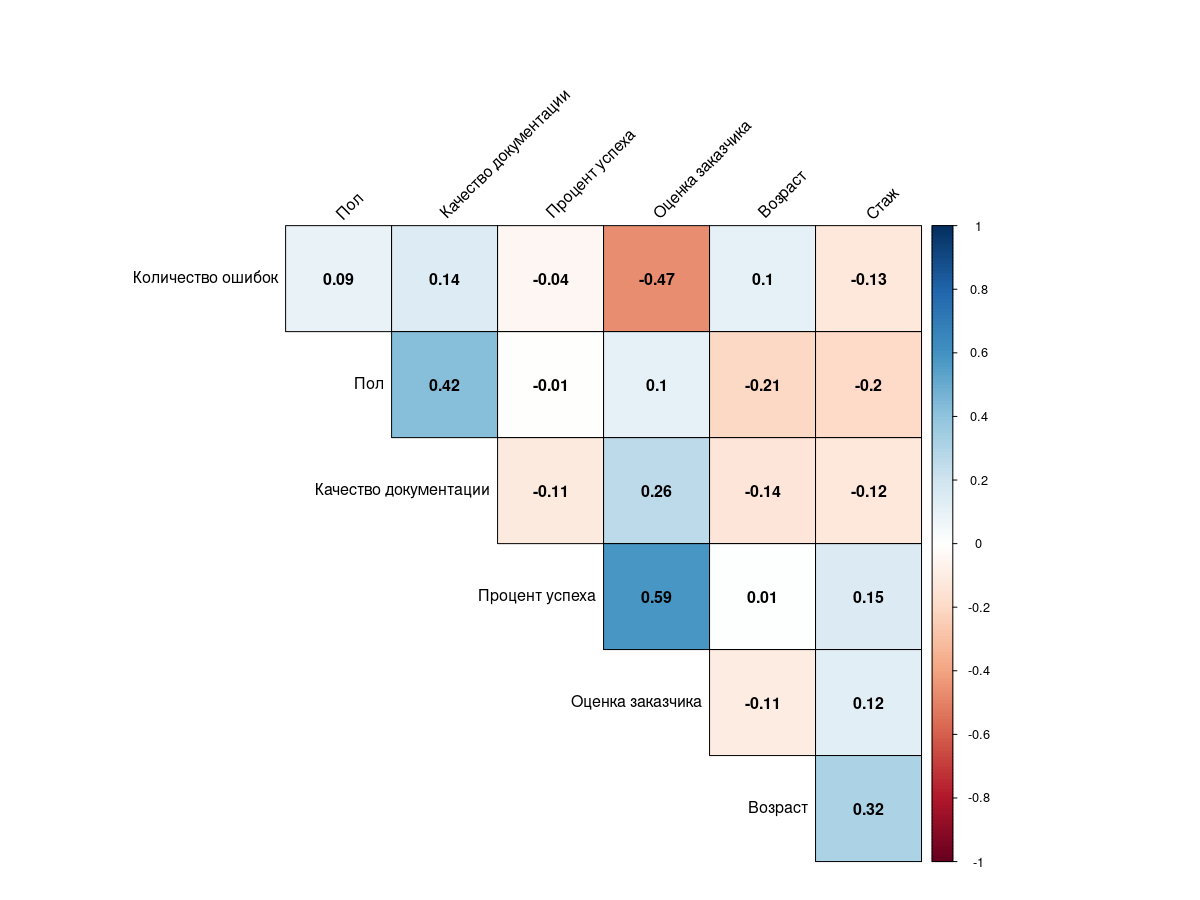
\includegraphics[width=\linewidth]{cor1}
	\caption{Матрица коэффициентов корреляции Пирсона для группы <<juniors>>}
	\label{cor1}
\end{figure}

\begin{figure}[H]
	\centering
	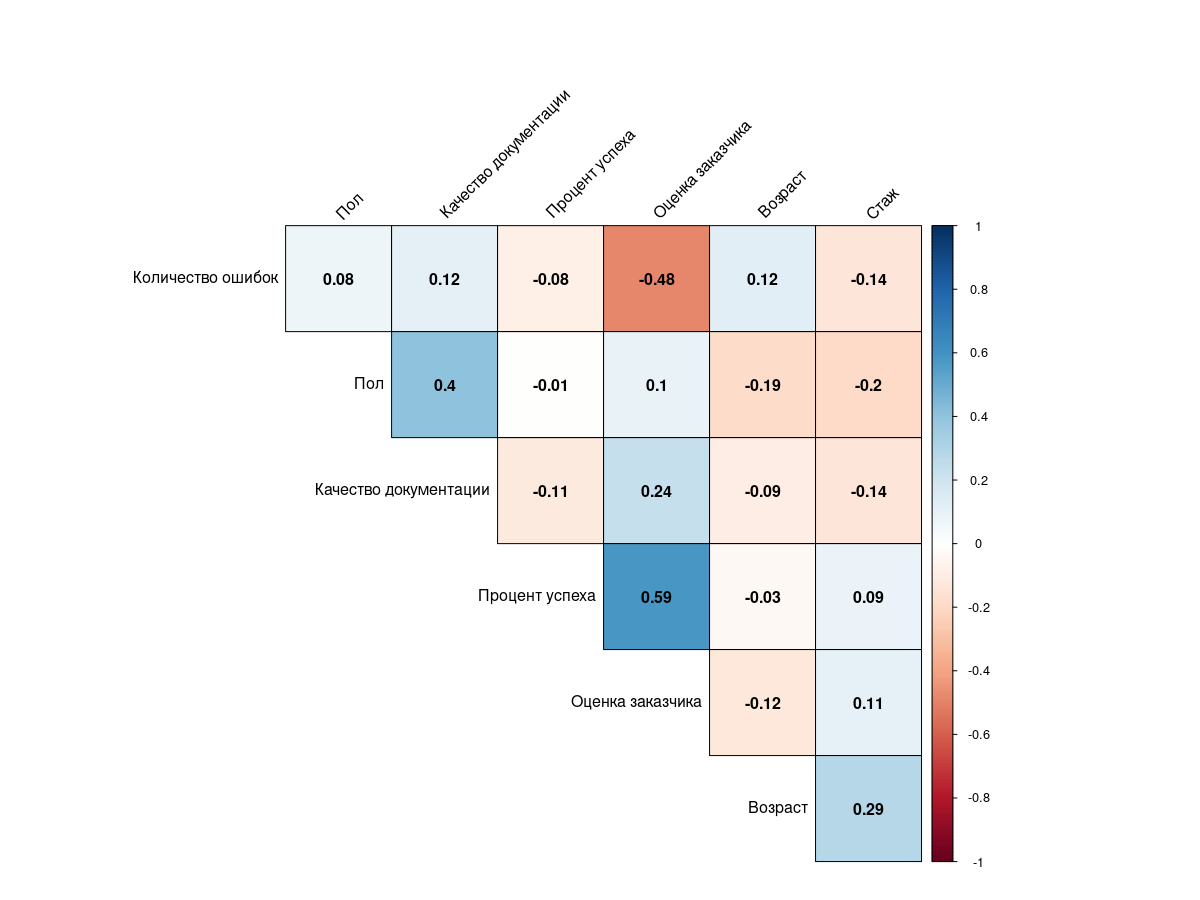
\includegraphics[width=\linewidth]{cor2}
	\caption{Матрица коэффициентов корреляции Спирмена для группы <<juniors>>}
	\label{cor2}
\end{figure}

\begin{figure}[H]
	\centering
	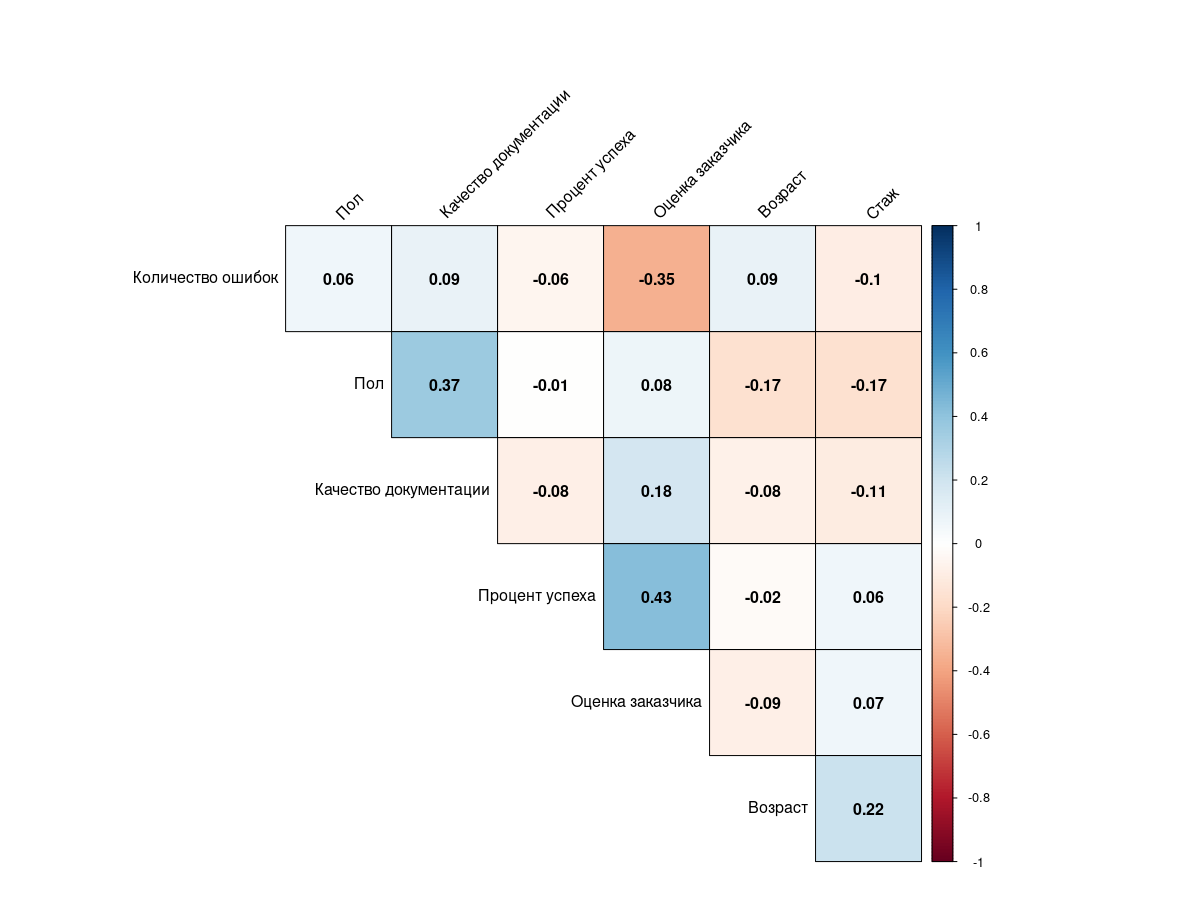
\includegraphics[width=\linewidth]{cor3}
	\caption{Матрица коэффициентов корреляции Канделла для группы <<juniors>>}
	\label{cor3}
\end{figure}



\begin{figure}[H]
	\centering
	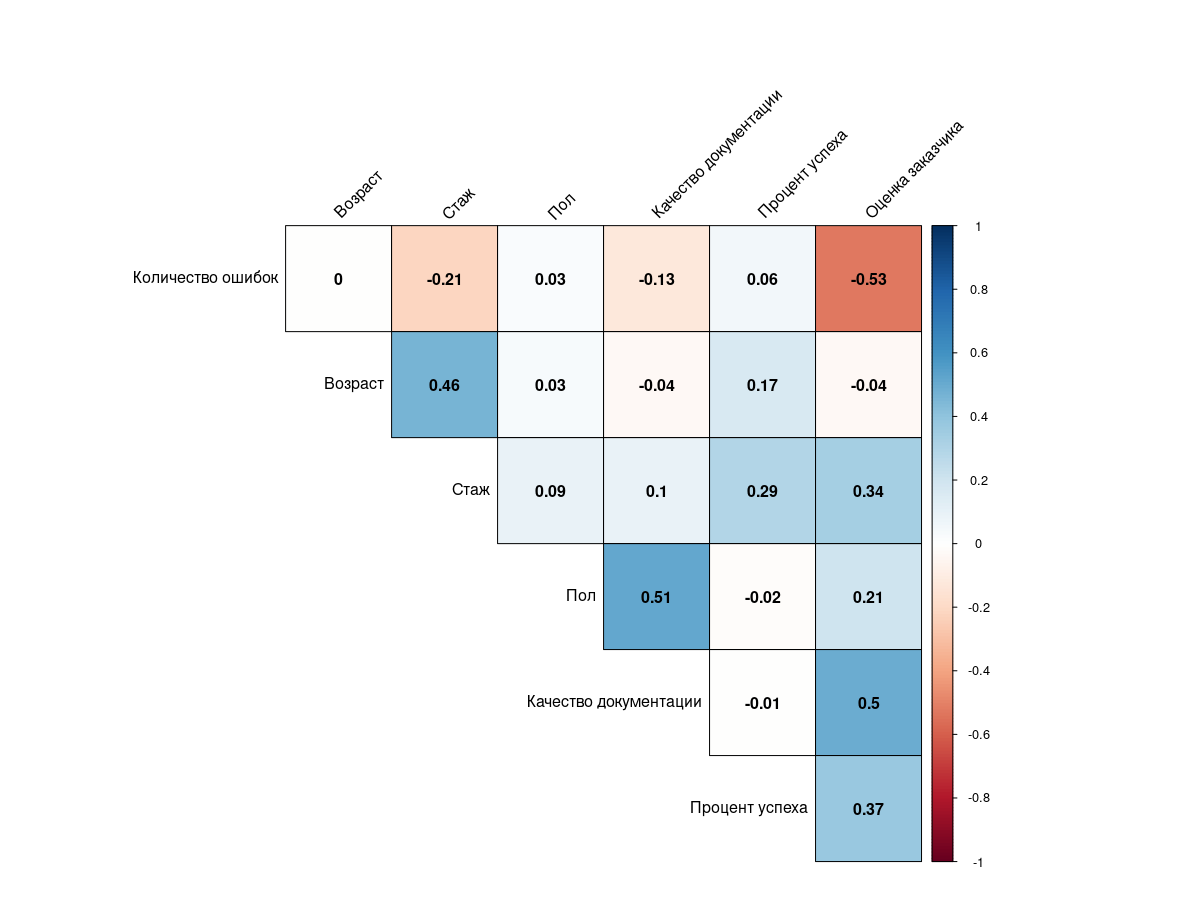
\includegraphics[width=\linewidth]{cor4}
	\caption{Матрица коэффициентов корреляции Пирсона для группы <<seniors>>}
	\label{cor4}
\end{figure}

\begin{figure}[H]
	\centering
	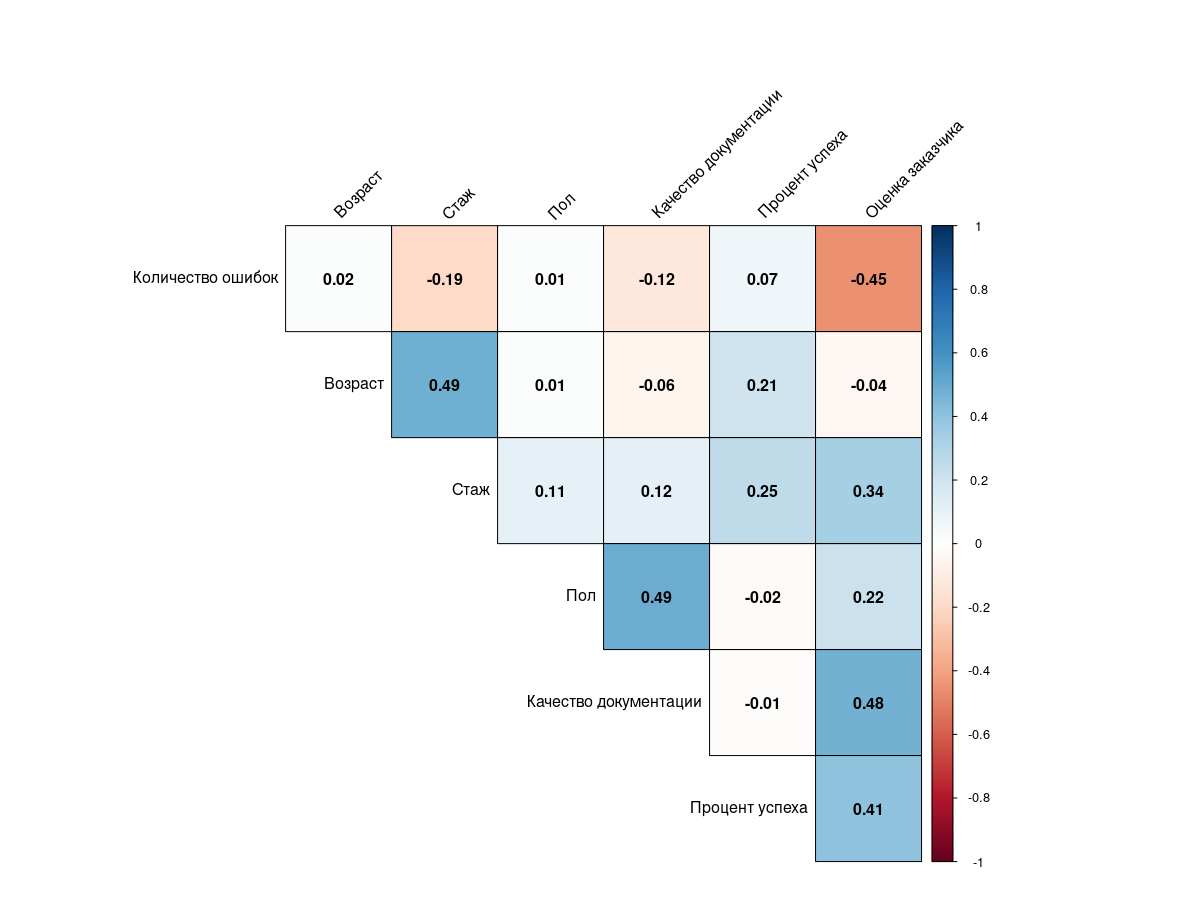
\includegraphics[width=\linewidth]{cor5}
	\caption{Матрица коэффициентов корреляции Спирмена для группы <<seniors>>}
	\label{cor5}
\end{figure}

\begin{figure}[H]
	\centering
	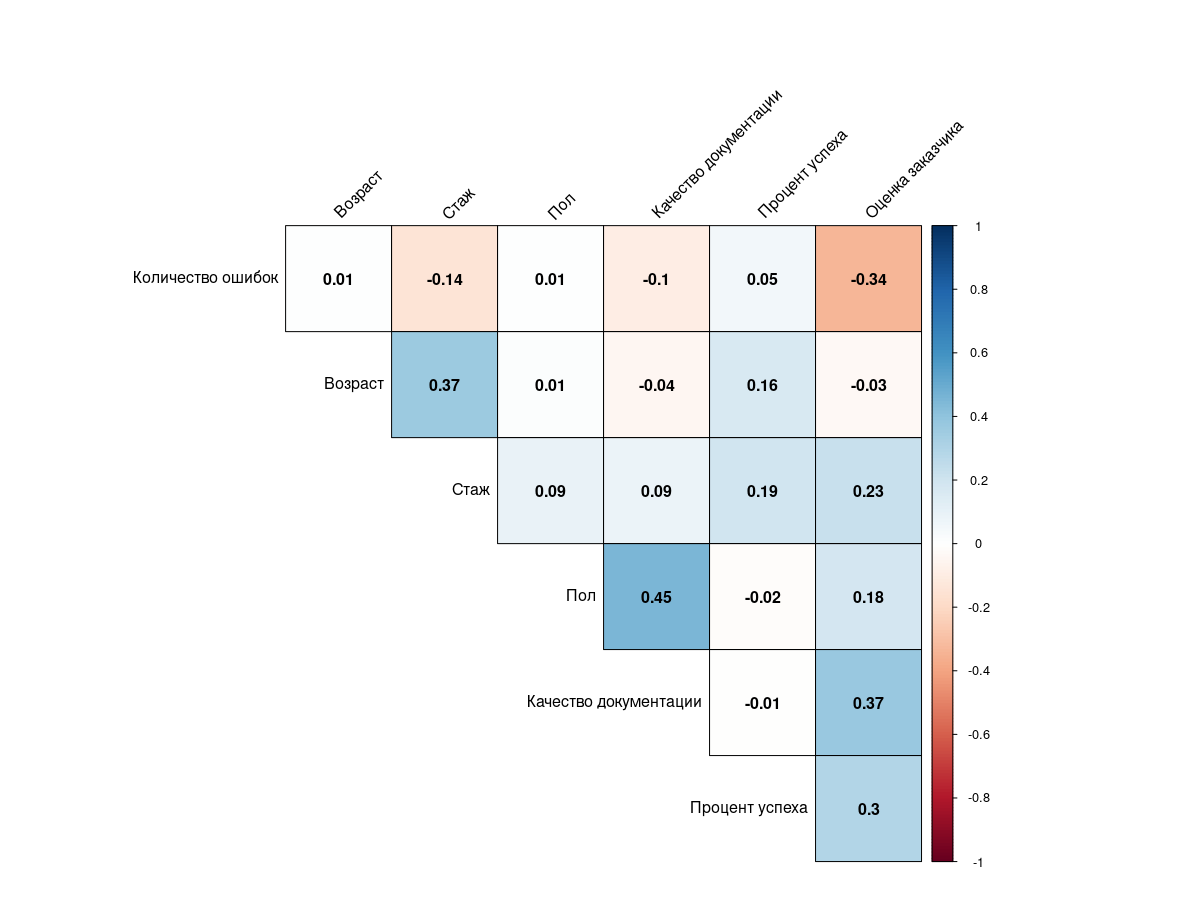
\includegraphics[width=\linewidth]{cor6}
	\caption{Матрица коэффициентов корреляции Канделла для группы <<seniors>>}
	\label{cor6}
\end{figure}


\subsection{Выводы}
Для обоих групп прослеживается наиболее сильная взаимосвязь между количеством допущенных ошибок и оценкой заказчика. Это можно объяснить тем, что каждый раз, когда заказчик обнаруживает ошибку, то он достаточно бурно реагирует, так как все неожиданно идет не так, как было запланировано изначально. Процент успеха, например, имеет меньшую связь с оценкой из-за того, что можно заранее предупредить заказчика о том, что часть какого-то функционала не будет готова в срок. Этот момент даст возможность заказчику подготовиться морально и на <<сошедших эмоциях>> выставить более высокую оценку.

Не коррелируют друг с другом, например, пол и количество ошибок, процент успеха и стаж.

\chapter{ЗАКЛЮЧЕНИЕ}

\section{Демонстрация работы}

\begin{figure}[H]
	\centering
	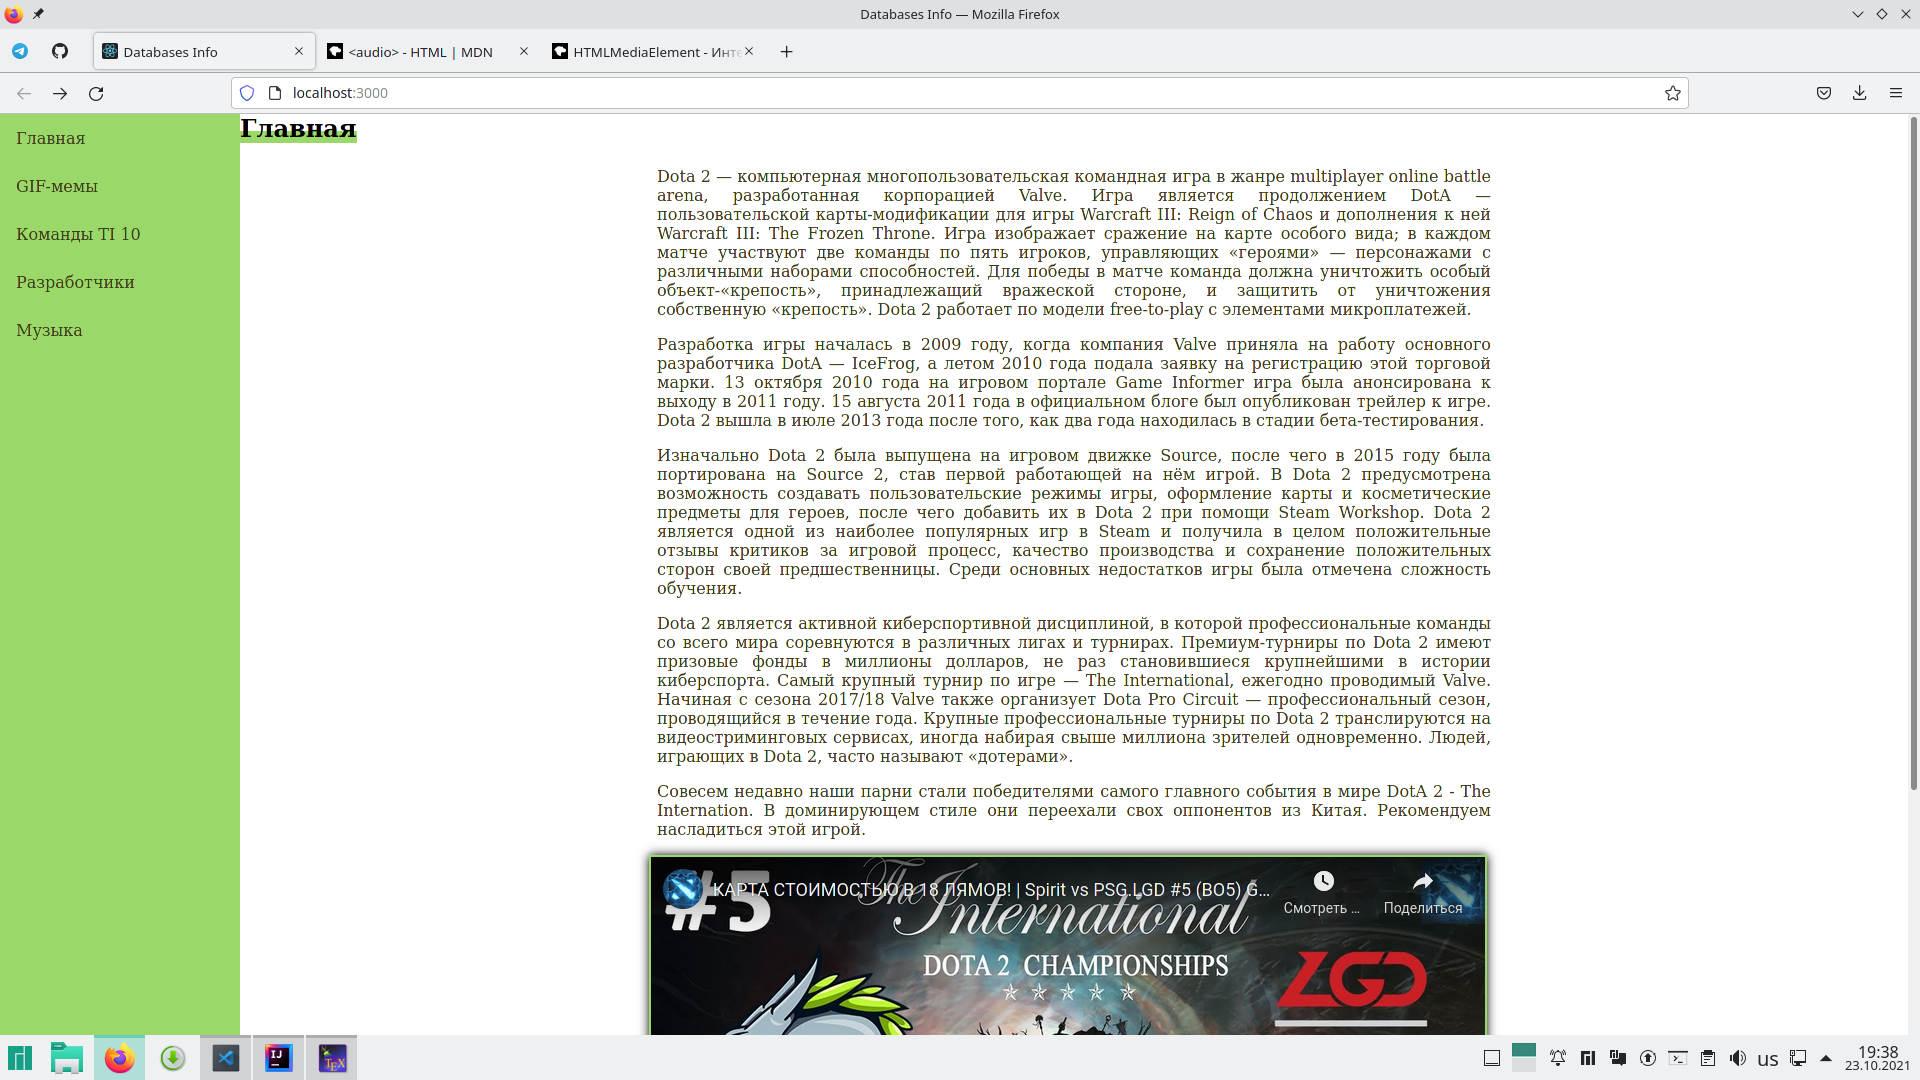
\includegraphics[width=0.7\textwidth]{01}
	\caption{Сохраненная база данных}
\end{figure}

\begin{figure}[H]
	\centering
	
\includegraphics[width=0.7\textwidth]{02}
	\caption{Файл JSON базы данных}
\end{figure}

\begin{figure}[H]
	\centering
	
\includegraphics[width=0.7\textwidth]{03}
	\caption{База данных после очистки}
\end{figure}

\begin{figure}[H]
	\centering
	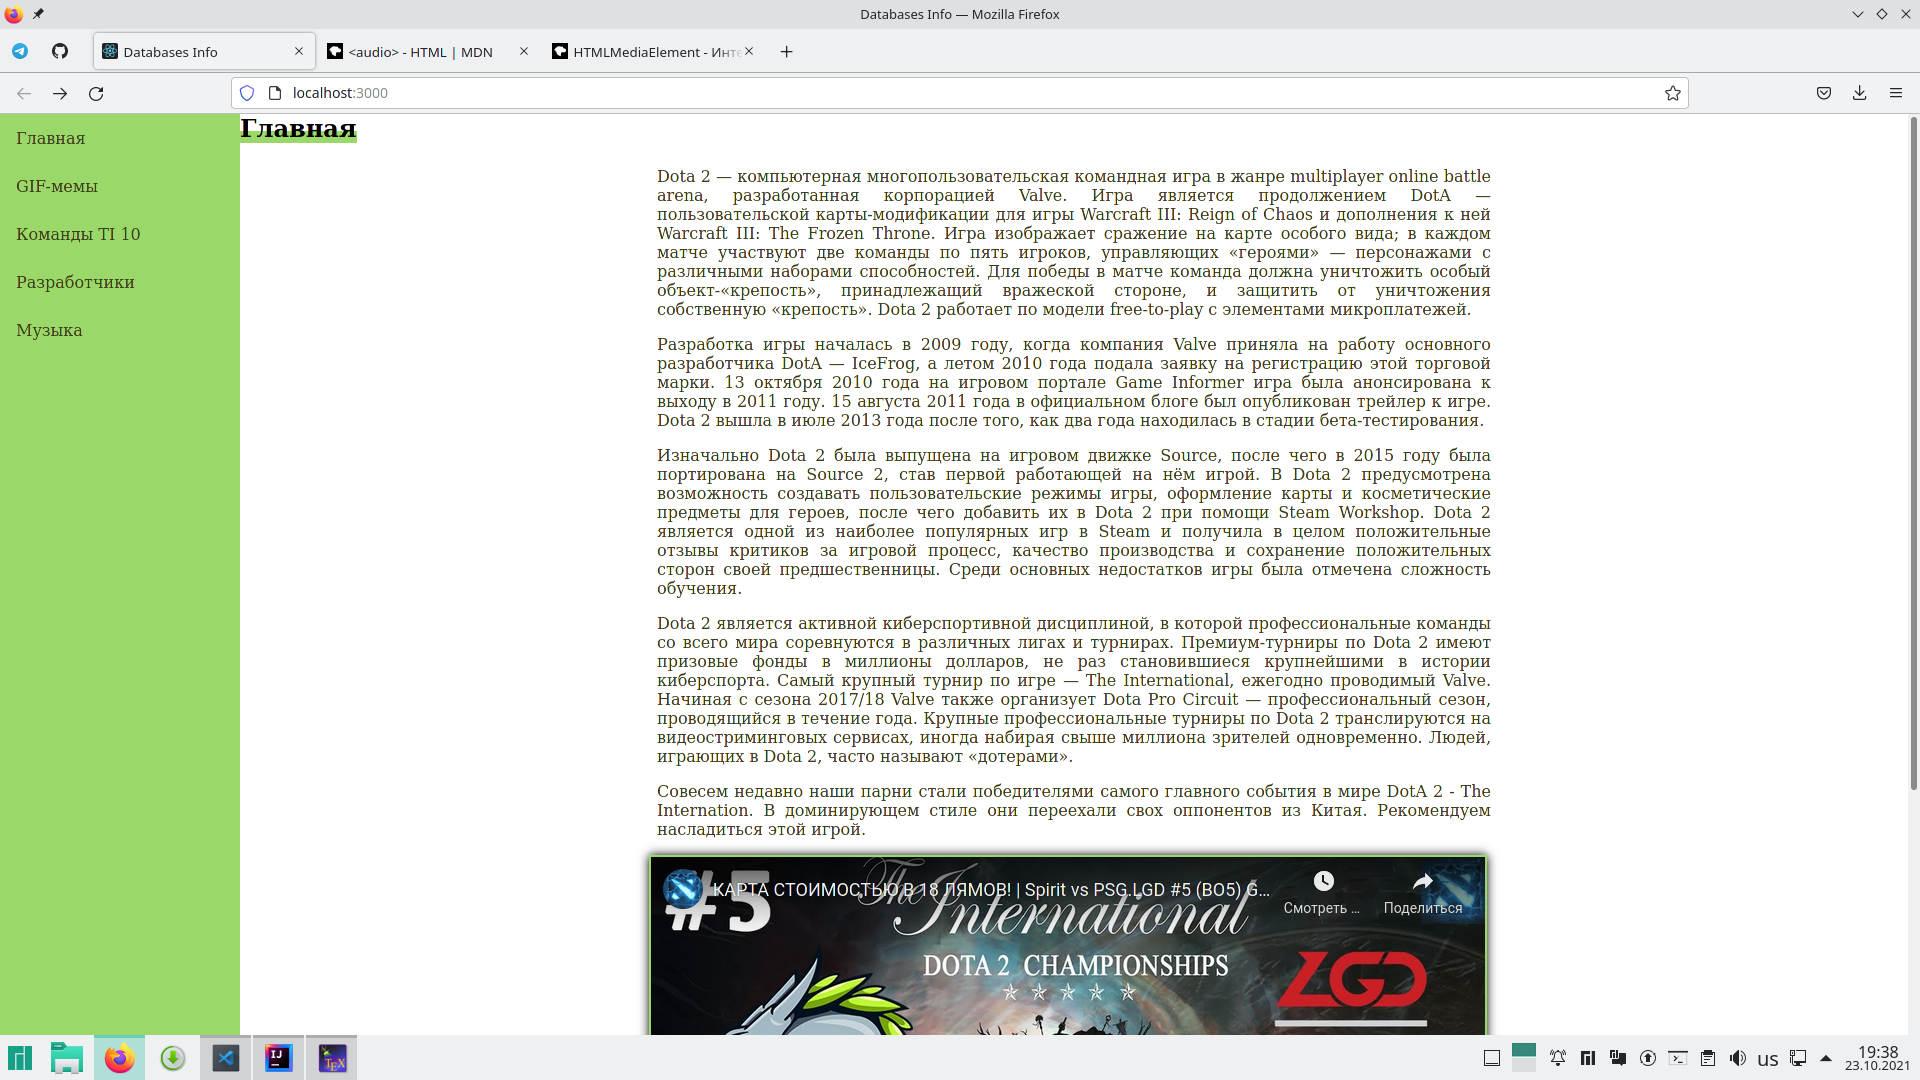
\includegraphics[width=0.7\textwidth]{01}
	\caption{База данных после восстановления}
\end{figure}

\section{Вывод}
В ходе выполнения лабораторной работы были реализованы:
\begin{enumerate}
	\item Запись данных из БД в файл формата JSON.
	\item Очистка данных из БД.
	\item Загрузка данных в БД из файла в формате JSON.
\end{enumerate}

\end{document}